\begin{figure}[h]
    \centering
    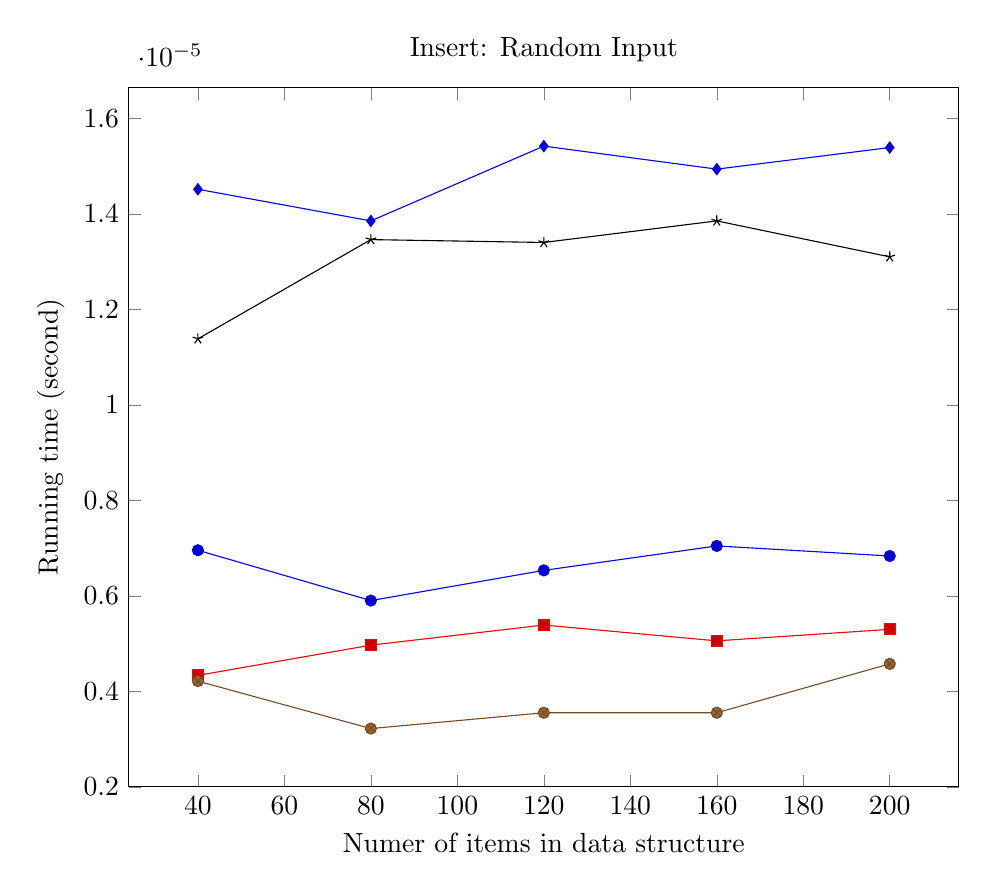
\begin{tikzpicture}
        \begin{axis}[
            xlabel={Numer of items in data structure},
            ylabel={Running time (second)},
            title={Insert: Random Input},
            width=\textwidth
        ]
		\addplot coordinates {
			(200, 6.836680144317598e-06)
			(160, 7.047502879942158e-06)
			(120, 6.535504807558823e-06)
			(80, 5.903036600329869e-06)
			(40, 6.957150278807944e-06)
		};
		\addplot coordinates {
			(200, 5.300685926812321e-06)
			(160, 5.059745657476355e-06)
			(120, 5.391038527946534e-06)
			(80, 4.969393056342142e-06)
			(40, 4.336924849113189e-06)
		};
		\addplot coordinates {
			(200, 4.577865118449153e-06)
			(160, 3.553868973327212e-06)
			(120, 3.5538689736824836e-06)
			(80, 3.222576103567576e-06)
			(40, 4.216454714622841e-06)
		};
		\addplot coordinates {
			(200, 1.310112714882905e-05)
			(160, 1.3854065490548351e-05)
			(120, 1.3402302485232554e-05)
			(80, 1.3462537553010633e-05)
			(40, 1.1384427729410618e-05)
		};
		\addplot coordinates {
			(200, 1.5390059708053626e-05)
			(160, 1.4938296703093101e-05)
			(120, 1.5420177241765032e-05)
			(80, 1.3854065490548351e-05)
			(40, 1.451665123148871e-05)
		};
        \legend{}
        \end{axis}
    \end{tikzpicture}
    \caption{Average of 0 operations, benchmarked every 0, starting at 0.}
\end{figure}